\documentclass{article}

% Official NeurIPS 2025 style (the latest released). [preprint] shows author names;
% the footer is replaced so the PDF does not claim to be a NeurIPS submission.
\PassOptionsToPackage{numbers,sort&compress}{natbib}
\usepackage[preprint]{neurips_2025}
\makeatletter
\renewcommand{\@noticestring}{ESE 5420 course project (University of Pennsylvania, Fall 2026), written in the format of a machine learning paper. Not peer reviewed.}
\makeatother

\usepackage[utf8]{inputenc}
\usepackage[T1]{fontenc}
\usepackage{hyperref}
\usepackage{url}
\usepackage{booktabs}
\usepackage{amsmath,amsfonts}
\usepackage{microtype}
\usepackage{xcolor}
\usepackage{graphicx}
\usepackage{capt-of}
\usepackage{float}
\hypersetup{colorlinks=true, linkcolor=black, citecolor=blue!50!black, urlcolor=blue!50!black}

% generated by src/make_tables.py
\newcommand{\LRcv}{0.56\%}
\newcommand{\LRcvse}{0.09\%}
\newcommand{\LRnested}{0.74\%}
\newcommand{\LRnestedse}{0.32\%}
\newcommand{\errGBTen}{21.00\%}
\newcommand{\errGBTwenty}{15.68\%}
\newcommand{\errGBThirty}{11.70\%}
\newcommand{\errGBFifty}{8.92\%}
\newcommand{\errGBHundred}{5.34\%}
\newcommand{\errGBOneFifty}{3.13\%}
\newcommand{\errGBTwoHundred}{1.91\%}
\newcommand{\errGBThreeHundred}{1.88\%}
\newcommand{\errGBFourHundred}{1.17\%}
\newcommand{\errGBSixHundred}{0.66\%}
\newcommand{\errGBEightHundred}{0.33\%}
\newcommand{\errLRTen}{16.28\%}
\newcommand{\errLRTwenty}{6.39\%}
\newcommand{\errLRThirty}{3.38\%}
\newcommand{\errLRFifty}{2.50\%}
\newcommand{\errLRHundred}{1.61\%}
\newcommand{\errLROneFifty}{1.22\%}
\newcommand{\errLRTwoHundred}{1.21\%}
\newcommand{\errLRThreeHundred}{1.07\%}
\newcommand{\errLRFourHundred}{0.93\%}
\newcommand{\errLRSixHundred}{0.82\%}
\newcommand{\errLREightHundred}{0.65\%}
\newcommand{\errNNTen}{11.90\%}
\newcommand{\errNNTwenty}{4.74\%}
\newcommand{\errNNThirty}{2.90\%}
\newcommand{\errNNFifty}{2.02\%}
\newcommand{\errNNHundred}{0.91\%}
\newcommand{\errNNOneFifty}{0.63\%}
\newcommand{\errNNTwoHundred}{0.49\%}
\newcommand{\errNNThreeHundred}{0.28\%}
\newcommand{\errNNFourHundred}{0.12\%}
\newcommand{\errNNSixHundred}{0.06\%}
\newcommand{\errNNEightHundred}{0.00\%}
\newcommand{\errRFTen}{23.24\%}
\newcommand{\errRFTwenty}{14.22\%}
\newcommand{\errRFThirty}{9.95\%}
\newcommand{\errRFFifty}{7.81\%}
\newcommand{\errRFHundred}{5.05\%}
\newcommand{\errRFOneFifty}{3.56\%}
\newcommand{\errRFTwoHundred}{2.41\%}
\newcommand{\errRFThreeHundred}{1.99\%}
\newcommand{\errRFFourHundred}{1.47\%}
\newcommand{\errRFSixHundred}{1.05\%}
\newcommand{\errRFEightHundred}{0.60\%}
\newcommand{\errKNNTen}{21.57\%}
\newcommand{\errKNNTwenty}{11.89\%}
\newcommand{\errKNNThirty}{7.11\%}
\newcommand{\errKNNFifty}{4.15\%}
\newcommand{\errKNNHundred}{1.60\%}
\newcommand{\errKNNOneFifty}{0.99\%}
\newcommand{\errKNNTwoHundred}{0.81\%}
\newcommand{\errKNNThreeHundred}{0.56\%}
\newcommand{\errKNNFourHundred}{0.31\%}
\newcommand{\errKNNSixHundred}{0.13\%}
\newcommand{\errKNNEightHundred}{0.13\%}
\newcommand{\diffGBTen}{+4.72}
\newcommand{\seGBTen}{1.81}
\newcommand{\winsGBTen}{18}
\newcommand{\diffGBTwenty}{+9.29}
\newcommand{\seGBTwenty}{1.20}
\newcommand{\winsGBTwenty}{6}
\newcommand{\diffGBThirty}{+8.32}
\newcommand{\seGBThirty}{0.65}
\newcommand{\winsGBThirty}{1}
\newcommand{\diffGBFifty}{+6.43}
\newcommand{\seGBFifty}{0.52}
\newcommand{\winsGBFifty}{1}
\newcommand{\diffGBHundred}{+3.74}
\newcommand{\seGBHundred}{0.38}
\newcommand{\winsGBHundred}{0}
\newcommand{\diffGBOneFifty}{+1.91}
\newcommand{\seGBOneFifty}{0.19}
\newcommand{\winsGBOneFifty}{2}
\newcommand{\diffGBTwoHundred}{+0.69}
\newcommand{\seGBTwoHundred}{0.13}
\newcommand{\winsGBTwoHundred}{12}
\newcommand{\diffGBThreeHundred}{+0.81}
\newcommand{\seGBThreeHundred}{0.15}
\newcommand{\winsGBThreeHundred}{7}
\newcommand{\diffGBFourHundred}{+0.24}
\newcommand{\seGBFourHundred}{0.08}
\newcommand{\winsGBFourHundred}{15}
\newcommand{\diffGBSixHundred}{-0.16}
\newcommand{\seGBSixHundred}{0.08}
\newcommand{\winsGBSixHundred}{27}
\newcommand{\diffGBEightHundred}{-0.32}
\newcommand{\seGBEightHundred}{0.08}
\newcommand{\winsGBEightHundred}{34}
\newcommand{\diffNNTen}{-4.39}
\newcommand{\seNNTen}{1.21}
\newcommand{\winsNNTen}{33}
\newcommand{\diffNNTwenty}{-1.65}
\newcommand{\seNNTwenty}{0.74}
\newcommand{\winsNNTwenty}{29}
\newcommand{\diffNNThirty}{-0.48}
\newcommand{\seNNThirty}{0.27}
\newcommand{\winsNNThirty}{30}
\newcommand{\diffNNFifty}{-0.47}
\newcommand{\seNNFifty}{0.15}
\newcommand{\winsNNFifty}{31}
\newcommand{\diffNNHundred}{-0.70}
\newcommand{\seNNHundred}{0.12}
\newcommand{\winsNNHundred}{44}
\newcommand{\diffNNOneFifty}{-0.59}
\newcommand{\seNNOneFifty}{0.08}
\newcommand{\winsNNOneFifty}{45}
\newcommand{\diffNNTwoHundred}{-0.72}
\newcommand{\seNNTwoHundred}{0.07}
\newcommand{\winsNNTwoHundred}{47}
\newcommand{\diffNNThreeHundred}{-0.80}
\newcommand{\seNNThreeHundred}{0.06}
\newcommand{\winsNNThreeHundred}{48}
\newcommand{\diffNNFourHundred}{-0.81}
\newcommand{\seNNFourHundred}{0.05}
\newcommand{\winsNNFourHundred}{50}
\newcommand{\diffNNSixHundred}{-0.75}
\newcommand{\seNNSixHundred}{0.06}
\newcommand{\winsNNSixHundred}{49}
\newcommand{\diffNNEightHundred}{-0.65}
\newcommand{\seNNEightHundred}{0.06}
\newcommand{\winsNNEightHundred}{45}
\newcommand{\diffRFTen}{+6.96}
\newcommand{\seRFTen}{1.46}
\newcommand{\winsRFTen}{13}
\newcommand{\diffRFTwenty}{+7.83}
\newcommand{\seRFTwenty}{0.98}
\newcommand{\winsRFTwenty}{5}
\newcommand{\diffRFThirty}{+6.57}
\newcommand{\seRFThirty}{0.46}
\newcommand{\winsRFThirty}{1}
\newcommand{\diffRFFifty}{+5.31}
\newcommand{\seRFFifty}{0.42}
\newcommand{\winsRFFifty}{1}
\newcommand{\diffRFHundred}{+3.44}
\newcommand{\seRFHundred}{0.35}
\newcommand{\winsRFHundred}{1}
\newcommand{\diffRFOneFifty}{+2.34}
\newcommand{\seRFOneFifty}{0.21}
\newcommand{\winsRFOneFifty}{0}
\newcommand{\diffRFTwoHundred}{+1.19}
\newcommand{\seRFTwoHundred}{0.16}
\newcommand{\winsRFTwoHundred}{8}
\newcommand{\diffRFThreeHundred}{+0.92}
\newcommand{\seRFThreeHundred}{0.13}
\newcommand{\winsRFThreeHundred}{5}
\newcommand{\diffRFFourHundred}{+0.55}
\newcommand{\seRFFourHundred}{0.10}
\newcommand{\winsRFFourHundred}{7}
\newcommand{\diffRFSixHundred}{+0.23}
\newcommand{\seRFSixHundred}{0.09}
\newcommand{\winsRFSixHundred}{19}
\newcommand{\diffRFEightHundred}{-0.04}
\newcommand{\seRFEightHundred}{0.08}
\newcommand{\winsRFEightHundred}{21}
\newcommand{\diffKNNTen}{+5.28}
\newcommand{\seKNNTen}{1.64}
\newcommand{\winsKNNTen}{16}
\newcommand{\diffKNNTwenty}{+5.50}
\newcommand{\seKNNTwenty}{1.12}
\newcommand{\winsKNNTwenty}{9}
\newcommand{\diffKNNThirty}{+3.73}
\newcommand{\seKNNThirty}{0.49}
\newcommand{\winsKNNThirty}{6}
\newcommand{\diffKNNFifty}{+1.66}
\newcommand{\seKNNFifty}{0.34}
\newcommand{\winsKNNFifty}{14}
\newcommand{\diffKNNHundred}{-0.01}
\newcommand{\seKNNHundred}{0.18}
\newcommand{\winsKNNHundred}{27}
\newcommand{\diffKNNOneFifty}{-0.23}
\newcommand{\seKNNOneFifty}{0.11}
\newcommand{\winsKNNOneFifty}{34}
\newcommand{\diffKNNTwoHundred}{-0.40}
\newcommand{\seKNNTwoHundred}{0.08}
\newcommand{\winsKNNTwoHundred}{37}
\newcommand{\diffKNNThreeHundred}{-0.51}
\newcommand{\seKNNThreeHundred}{0.08}
\newcommand{\winsKNNThreeHundred}{40}
\newcommand{\diffKNNFourHundred}{-0.61}
\newcommand{\seKNNFourHundred}{0.05}
\newcommand{\winsKNNFourHundred}{45}
\newcommand{\diffKNNSixHundred}{-0.68}
\newcommand{\seKNNSixHundred}{0.06}
\newcommand{\winsKNNSixHundred}{48}
\newcommand{\diffKNNEightHundred}{-0.52}
\newcommand{\seKNNEightHundred}{0.06}
\newcommand{\winsKNNEightHundred}{41}
\newcommand{\reachGBTwo}{195}
\newcommand{\reachGBOne}{446}
\newcommand{\reachLRTwo}{71}
\newcommand{\reachLROne}{345}
\newcommand{\reachNNTwo}{50}
\newcommand{\reachNNOne}{92}
\newcommand{\reachRFTwo}{297}
\newcommand{\reachRFOne}{614}
\newcommand{\reachKNNTwo}{85}
\newcommand{\reachKNNOne}{149}
\newcommand{\gerrLRFifty}{2.30\%}
\newcommand{\gerrLRHundred}{1.86\%}
\newcommand{\gerrLRTwoHundred}{1.14\%}
\newcommand{\gerrLRFourHundred}{0.96\%}
\newcommand{\gerrLREightHundred}{0.71\%}
\newcommand{\gerrKNNFifty}{4.53\%}
\newcommand{\gerrKNNHundred}{1.57\%}
\newcommand{\gerrKNNTwoHundred}{0.74\%}
\newcommand{\gerrKNNFourHundred}{0.30\%}
\newcommand{\gerrKNNEightHundred}{0.13\%}
\newcommand{\testLR}{0.37\%}
\newcommand{\testerrLR}{1}
\newcommand{\testKNN}{0.37\%}
\newcommand{\testerrKNN}{1}
\newcommand{\testRF}{1.11\%}
\newcommand{\testerrRF}{3}
\newcommand{\testGB}{0.37\%}
\newcommand{\testerrGB}{1}
\newcommand{\testNN}{0.00\%}
\newcommand{\testerrNN}{0}


\title{How Many Training Notes? Sample Efficiency of Linear, Nearest-Neighbour, Tree and Neural Classifiers for Forged-Banknote Detection}

\author{Maanas \qquad Advit \\ University of Pennsylvania}

\begin{document}
\maketitle

\begin{abstract}
On the UCI Banknote Authentication benchmark, a tuned logistic regression already misclassifies only \LRcv{} of notes in cross-validation, so ranking methods by final accuracy compares noise. We instead ask how many labelled training notes each method needs. We compare logistic regression (the baseline) and $k$-nearest neighbours, with random forests, gradient boosting and a small neural network as extensions, along learning curves from 10 to 800 training notes. Each size has 50 paired draws, and every method is tuned by cross-validation inside each draw. Logistic regression learns fastest of the core methods at first (2\% error from about \reachLRTwo{} notes) but levels off near 0.6\%. $k$NN overtakes it at about 100 notes and reaches 1\% error from about \reachKNNOne{} notes, against \reachLROne{}. Tree ensembles are the slowest learners, while an 8-unit neural network has the lowest error at every size and reaches 1\% from about \reachNNOne{} notes. A check for several images of the same physical specimen leaves these results unchanged. On the 270-note test set, all methods make 0--3 errors and are statistically tied, which is why the learning curves, not the test set, carry the comparison.
\end{abstract}

\section{Introduction}
\label{sec:intro}
Counterfeit detection is a natural use for a cheap classifier. A scanner photographs a note, a few image statistics are computed, and a model flags it as genuine or forged. The UCI Banknote Authentication data \cite{lohweg2012uci} is a standard small benchmark for this task, with four wavelet features per image. On it, standard methods are almost perfect: a tuned logistic regression misclassifies \LRcv{} of notes in 5-fold cross-validation (CV). Ranking methods by their final accuracy here would mostly compare noise, because with a few hundred held-out notes the difference between 0.3\% and 0.6\% error is one or two notes.

We therefore ask a question that still separates methods when accuracy saturates: \emph{how many labelled training notes does each method need to reach a given error rate?} In practice, labelled forgeries are the expensive part of building such a system, because each one must be produced or seized and then verified. A method that reaches 1\% error from 100 notes is more useful than one that needs 800, even if both are perfect at 1,000.

We compare two methods taught early in the course, logistic regression (the baseline) and $k$-nearest neighbours ($k$NN), and three later ones as an extension: random forests, gradient boosting and a one-hidden-layer neural network. We draw learning curves from 10 to 800 training notes with 50 random draws per size, tune every method by CV inside each draw, and compare methods on the same draws. Our contributions are:
\begin{itemize}
  \item a leakage-aware protocol for this dataset: duplicate removal, scaling and tuning inside each training set, an untouched test set, and a check for several images of the same physical specimen;
  \item paired learning curves with standard errors, and the number of notes each method needs to reach 2\% and 1\% error, with bootstrap intervals;
  \item an honest reading of where the differences are real and where they are ties, including the one-time test-set result.
\end{itemize}
Among the two core methods we find a crossover. Logistic regression learns fastest at first, reaching 2\% error from about \reachLRTwo{} notes, but levels off near 0.6\% because no linear boundary separates the classes. $k$NN starts worse, catches up at about 100 notes and reaches 1\% from about \reachKNNOne{} notes, against \reachLROne{} for logistic regression. Among the extensions, the tree ensembles are the least sample-efficient methods we tried, while a small neural network with 8 hidden units has the lowest mean error at every size from 10 notes up and reaches 1\% from about \reachNNOne{} notes. On the 270 test notes, all five methods make between 0 and 3 errors, so the test set cannot separate them; the learning curves can.

\section{Related work}
\label{sec:related}
\paragraph{Dataset.} The data come from the authentication work of Gillich and Lohweg \cite{gillich2010banknote}: images of genuine and forged banknote-like specimens were taken with an industrial camera and summarised by statistics of a wavelet transform. Lohweg released the four features on the UCI repository \cite{lohweg2012uci}. Because most standard methods score close to 100\% on it, a single accuracy figure says little about which method to prefer.

\paragraph{Learning curves for comparing classifiers.} Perlich, Provost and Simonoff \cite{perlich2003tree} compared logistic regression and tree induction across training sizes in a large-scale study of many datasets. They found that logistic regression tends to win on small samples and trees on large ones, so that the curves can cross and a comparison at one size can mislead. Ng and Jordan \cite{ng2002discriminative} showed a related effect between generative and discriminative models: the method with the lower asymptotic error is not always the faster learner. Viering and Loog \cite{viering2023shape} review the shapes learning curves take, including non-monotone ones. Our study applies this learning-curve view to a dataset where final accuracy is saturated.

\paragraph{Fair evaluation.} Choosing hyperparameters and estimating error on the same folds biases the estimate downwards \cite{varma2006bias,cawley2010overfitting}, so we use nested CV for the baseline and tune inside every training draw. Leakage between training and evaluation data, for example near-copies of the same object, can make a model look better than it is \cite{kaufman2012leakage}. To compare two classifiers on one test set we use McNemar's test, as recommended by Dietterich \cite{dietterich1998approximate}.

\paragraph{Methods.} We use standard forms of logistic regression and CV \cite{james2021isl}, nearest-neighbour classification \cite{cover1967nearest}, random forests \cite{breiman2001random}, gradient boosting \cite{friedman2001greedy} and a small multilayer perceptron, all in scikit-learn \cite{pedregosa2011scikit}.

\section{Data}
\label{sec:data}
The UCI file \cite{lohweg2012uci} (CC BY 4.0) has 1,372 rows. Each has four inputs, the variance, skewness, kurtosis and entropy of a wavelet-transformed image, and a binary class. There are no missing values. We remove 24 exact duplicate rows, all from class 0, which leaves 1,348 notes, 45.3\% of them in class 1 (Table~\ref{tab:data}). UCI does not say which class is forged, and secondary sources disagree, so we call class 1 ``forged''. Error and AUC do not depend on this choice; missed forgeries and false alarms would swap.

\begin{table}[t]
  \centering
  \caption{Data size and shape at each stage. ``Forged'' is the share of class 1.}
  \label{tab:data}
  \small
  % generated by src/make_tables.py
\begin{tabular}{lrrr}
\toprule
Stage & Rows & Inputs & Forged \\
\midrule
Raw UCI file & 1372 & 4 & 44.5\% \\
After removing exact duplicates & 1348 & 4 & 45.3\% \\
Development set (80\%) & 1078 & 4 & 45.3\% \\
Test set (20\%, held out) & 270 & 4 & 45.2\% \\
\bottomrule
\end{tabular}
% 24 duplicate rows dropped

\end{table}

We make one stratified 80/20 split with a fixed random seed\footnote{The seed is 5420, the course number. It is only a fixed starting point for the random-number generator, so that anyone rerunning the code gets the same split; it was not chosen by looking at results. Every later random choice derives its seed from it.} into 1,078 development notes and 270 test notes, and store it with the data. All tuning, learning curves and model choices use the development notes only. The test notes were used once, after every modelling choice was fixed (Section~\ref{sec:test}).

\paragraph{Several images per specimen?} The file has no specimen identifiers, but the class-1 rows are strongly correlated in file order: the lag-1 autocorrelation of skewness is 0.62 for class 1 and about 0 for class 0, with a repeating pattern roughly every 8 rows. This suggests that the forged class contains several images of each physical specimen in a row. If near-identical images of one note fall on both sides of a split, a method that memorises training points, such as 1-nearest-neighbour, gains an unfair advantage. We cannot remove this risk without identifiers, so we test for it: we treat each run of 8 consecutive rows of one class as a pseudo-specimen and repeat the key experiments with whole pseudo-specimens kept on one side of every split (Section~\ref{sec:grouped}).

\section{Method}
\label{sec:method}
\paragraph{Classifiers.} All inputs are standardised inside each training set (a scikit-learn pipeline \cite{pedregosa2011scikit}), so no statistics leak from evaluation rows. Each method has a small grid tuned by stratified 5-fold CV on the training set alone:
\begin{itemize}
  \item \textbf{Logistic regression} (baseline): $C\in\{10^{-3},10^{-2.5},\dots,10^{3}\}$, 13 values.
  \item \textbf{$k$NN}: $k\in\{1,3,5,7,9,11,15,21,31\}$, limited to $k$ smaller than an inner training fold.
  \item \textbf{Random forest}$^\dagger$: 200 trees; features per split $m\in\{1,2,4\}$, minimum leaf size $\in\{1,3\}$.
  \item \textbf{Gradient boosting}$^\dagger$: 200 trees; learning rate $\eta\in\{0.05,0.2\}$, depth $\in\{1,3\}$.
  \item \textbf{Neural network}$^\dagger$: one hidden layer with 8 or 32 ReLU units, weight decay $\alpha\in\{10^{-4},10^{-2},1\}$, trained by L-BFGS.
\end{itemize}
$^\dagger$Later-course extensions (ensembles and neural networks). No baseline number depends on them. The grids are deliberately small so that every method can be tuned inside each of 2,750 training draws. Appendix~\ref{app:forest} shows that a 64-setting forest grid on all development data does not do better than the small one.

\paragraph{Baseline estimate.} On all 1,078 development notes we report the 5-fold CV error of logistic regression at the chosen $C$, with the standard error (SE) of the five fold errors, SD$/\sqrt{5}$. Because $C$ is chosen on the same folds, we also report nested 5$\times$5 CV.

\paragraph{Learning curves.} For each training size $n\in\{10,20,30,50,100,150,200,300,400,600,800\}$ and each of 50 draws, we sample $n$ development notes stratified by class, tune each method by 5-fold CV inside the sample, and score it on all remaining development notes (between 278 and 1,068). All methods see the same 50 training sets at each size, so we compare them with paired differences: for method $j$ and draw $d$, $\Delta_{jd}=\text{err}_{jd}-\text{err}_{\text{LR},d}$, reported as the mean over draws $\pm$ its SE. We call a difference clear when it exceeds 2 SE.

\paragraph{Notes needed to reach a target.} For each method we find where the mean curve first falls to 2\% and to 1\% error, by linear interpolation between neighbouring sizes on log--log axes. We get a 95\% interval by resampling the 50 draws at every size with replacement (2,000 bootstrap replicates) and repeating the calculation.

\paragraph{Test evaluation.} Each method is tuned by 5-fold CV on all development notes, refitted on them, and scored once on the 270 test notes. We give Wilson 95\% intervals for each error, and compare each method with the baseline by an exact McNemar test on the notes where the two disagree \cite{dietterich1998approximate}.

\section{Experiments and results}
\label{sec:results}

\subsection{Baseline}
On all 1,078 development notes, logistic regression chooses $C=100$, almost no regularisation, and reaches a 5-fold CV error of \LRcv{} $\pm$ \LRcvse{}: 6 wrong notes. Nested CV, which also accounts for choosing $C$, gives \LRnested{} $\pm$ \LRnestedse{} (Appendix~\ref{app:baseline}). The majority-class rule errs on 45.3\%. Even without regularisation, logistic regression still gets 4 of its own training notes wrong, so the classes are not linearly separable in these features. The baseline's remaining error is therefore bias, not a lack of data, and that already predicts how its learning curve will look.

\subsection{Learning curves}
\label{sec:curves}
\begin{figure}[t]
  \centering
  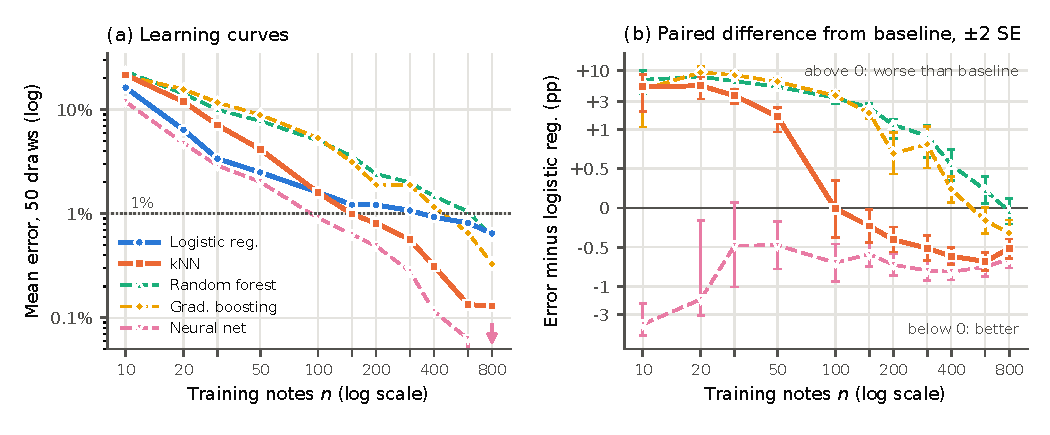
\includegraphics[width=\linewidth]{../figures/learning_curves.pdf}
  \caption{(a) Mean error on held-out development notes over 50 draws per size (log--log). Solid lines are the core methods, dashed lines the later-course extensions. The arrow marks the neural network at $n=800$, where all 50 draws had zero errors. (b) Paired difference from logistic regression on the same draws, in percentage points, with $\pm$2 SE bars (symmetric-log axis, linear between $-1$ and $+1$). Below 0 is better than the baseline.}
  \label{fig:curves}
\end{figure}

Figure~\ref{fig:curves} shows the main result; full numbers are in Appendix~\ref{app:full}.

\paragraph{Logistic regression vs.\ $k$NN.} Logistic regression is clearly better at small sizes: at 50 notes it errs on \errLRFifty{} against \errKNNFifty{} for $k$NN, a paired gap of \diffKNNFifty{} $\pm$ \seKNNFifty{} points. The two tie at 100 notes (\errLRHundred{} vs.\ \errKNNHundred{}). From 150 notes $k$NN is clearly better (\diffKNNOneFifty{} $\pm$ \seKNNOneFifty{} points) and the gap keeps growing, because logistic regression flattens out while $k$NN does not: at 800 notes the errors are \errLREightHundred{} and \errKNNEightHundred{}, and $k$NN wins \winsKNNEightHundred{} of 50 draws. Inner CV picks $k=1$ in most draws at every size (Table~\ref{tab:params}). This matches the crossing curves Perlich et al.\ \cite{perlich2003tree} report for logistic regression against a more flexible learner, which has the lower error at large sizes but needs more data to get there.

\paragraph{Extensions.} The two tree ensembles are worse than the baseline at every size up to 400 notes, often by several points: at 100 notes the forest errs on \errRFHundred{} and boosting on \errGBHundred{}. Boosting is clearly better than the baseline only at 800 notes (\errGBEightHundred{}), and the forest only ties it there. A larger forest grid on all development notes does not help (Appendix~\ref{app:forest}), so this is not a tuning problem. The small neural network, in contrast, has the lowest mean error of all five methods at every size. At 10 notes it errs on \errNNTen{} against \errLRTen{} for the baseline (\diffNNTen{} $\pm$ \seNNTen{} points), and at 800 notes none of its 50 draws makes a single error. CV most often picks the 8-unit network with weak weight decay.

\begin{figure}[t]
  \begin{minipage}[b]{0.44\linewidth}
    \centering
    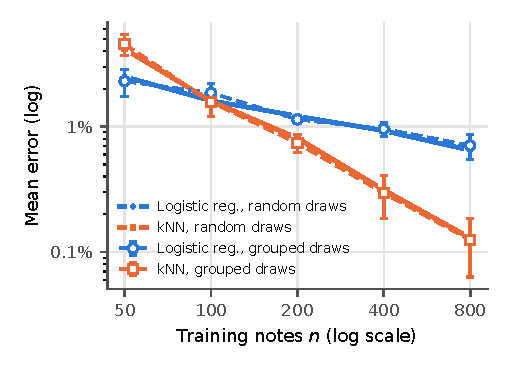
\includegraphics[width=\linewidth]{../figures/grouped.pdf}
    \captionof{figure}{Random draws (solid) vs.\ draws that keep each 8-row pseudo-specimen on one side of every split (dashed, $\pm$2 SE).}
    \label{fig:grouped}
  \end{minipage}\hfill
  \begin{minipage}[b]{0.53\linewidth}
    \centering
    \captionof{table}{Training notes needed for the mean error to reach 2\% and 1\%, interpolated on the learning curves, with bootstrap 95\% intervals over draws. $^\dagger$Extension.}
    \label{tab:reach}
    \small
    \setlength{\tabcolsep}{4pt}
    % generated by src/make_tables.py
\begin{tabular}{lrcrc}
\toprule
Method & \multicolumn{2}{c}{2\% error} & \multicolumn{2}{c}{1\% error} \\
 & $n$ & 95\% CI & $n$ & 95\% CI \\
\midrule
Logistic regression & 71 & 58--83 & 345 & 278--415 \\
$k$NN & 85 & 77--95 & 149 & 131--176 \\
Random forest$^\dagger$ & 297 & 247--326 & 614 & 560--648 \\
Gradient boosting$^\dagger$ & 195 & 184--304 & 446 & 403--479 \\
Neural network$^\dagger$ & 50 & 41--58 & 92 & 80--108 \\
\bottomrule
\end{tabular}

    \vspace{14pt}
  \end{minipage}
\end{figure}

\paragraph{Notes needed to reach a target.} Table~\ref{tab:reach} turns the curves into the quantity a practitioner would ask for. To reach 2\% error, the neural network needs about \reachNNTwo{} notes and logistic regression \reachLRTwo{}, with $k$NN close behind at \reachKNNTwo{}. To reach 1\%, the order changes: the neural network needs about \reachNNOne{}, $k$NN \reachKNNOne{}, and logistic regression \reachLROne{}, more than twice as many as $k$NN. The forest needs the most at both targets. The bootstrap intervals for the core methods do not overlap at 1\%.

\subsection{Several images per specimen}
\label{sec:grouped}
If $k$NN with $k=1$ wins only because it finds a near-copy of the same physical note in the training set, its advantage should shrink when whole pseudo-specimens are kept on one side of the split. It does not (Figure~\ref{fig:grouped}, Table~\ref{tab:grouped}). With grouped draws, $k$NN errs on \gerrKNNTwoHundred{} at 200 notes and \gerrKNNEightHundred{} at 800, against \errKNNTwoHundred{} and \errKNNEightHundred{} with random draws; logistic regression moves from \errLREightHundred{} to \gerrLREightHundred{} at 800. Grouped 5-fold CV on all development notes gives the same picture (Section~\ref{sec:data}; logistic regression 0.65\% and $k$NN 0.09\% in both cases). Within the limits of our heuristic grouping, the crossover is not an artefact of specimen leakage.

\subsection{Held-out test set}
\label{sec:test}
\begin{table}[t]
  \centering
  \caption{One-time evaluation on the 270 test notes (122 forged), after tuning by 5-fold CV on all development notes. ``Missed'' are forged notes called genuine, ``False al.'' genuine notes called forged. The interval is a Wilson 95\% interval; $p$ is an exact McNemar test against logistic regression. $^\dagger$Extension.}
  \label{tab:test}
  \small
  \setlength{\tabcolsep}{4.5pt}
  % generated by src/make_tables.py
\begin{tabular}{lrrrcrrcr}
\toprule
Method & Dev CV (\%) & Errors & Test (\%) & 95\% CI & Missed & False al. & AUC & $p$ vs LR \\
\midrule
Logistic regression & 0.56 & 1/270 & 0.37 & 0.1--2.1 & 0 & 1 & 0.9999 & -- \\
$k$NN & 0.09 & 1/270 & 0.37 & 0.1--2.1 & 0 & 1 & 0.9966 & 1.00 \\
Random forest$^\dagger$ & 0.56 & 3/270 & 1.11 & 0.4--3.2 & 0 & 3 & 0.9998 & 0.62 \\
Gradient boosting$^\dagger$ & 0.28 & 1/270 & 0.37 & 0.1--2.1 & 0 & 1 & 0.9999 & 1.00 \\
Neural network$^\dagger$ & 0.00 & 0/270 & 0.00 & 0.0--1.4 & 0 & 0 & 1.0000 & 1.00 \\
\bottomrule
\end{tabular}

\end{table}

Table~\ref{tab:test} gives the result of the single test evaluation. Logistic regression, $k$NN and boosting each misclassify \testerrLR{} of 270 notes (\testLR{}), the forest \testerrRF{}, and the neural network none. Every error is a false alarm; no method misses a forgery. These counts are too small to rank the methods: the 95\% intervals overlap heavily, and no McNemar test against the baseline comes close to significance ($p\ge0.62$). This is the outcome we expected before running it, and it is why the learning curves, not the test set, carry our conclusions. ROC curves are in Appendix~\ref{app:roc}.

\section{Discussion and limitations}
\label{sec:discussion}
\paragraph{Why the curves look the way they do.} We think the ranking follows the shape of decision boundary each method can represent. The evidence points to a smooth, curved boundary: no plane separates the development notes, but the 8-unit network separates all of them (0.00\% CV error on the full development set, Table~\ref{tab:test}). Logistic regression fits a plane with five parameters, so it is reliable from few notes but cannot get below its bias floor of about 0.6\%. $k$NN with $k=1$ can follow any boundary, but it needs enough notes to fill the space near it, so it starts badly and improves steadily. Trees split on one feature at a time, so they approximate a smooth oblique boundary with many small steps, and that needs many notes. The small neural network sits in between: with 8 hidden units (49 weights) it can represent a smooth curved boundary, yet it has far fewer degrees of freedom than $k$NN or a forest. On this dataset that appears to be the right inductive bias at every sample size we tried, although we did not test this explanation directly.

\paragraph{What a practitioner should take away.} If only a few dozen labelled notes are available, logistic regression or a small neural network is the safe choice; $k$NN and tree ensembles should not be used below about 100 notes. With a few hundred notes, the gap between the methods is a fraction of a percentage point, and the choice can be made on other grounds, such as interpretability (logistic regression) or simplicity ($k$NN). The answer to ``which method is best?'' depends on $n$, which a single accuracy number hides.

\subsection*{Limitations}
\begin{itemize}
  \item \textbf{One dataset, four features.} The conclusions are about this benchmark. They are not a claim about real currency authentication, where the notes, scanners and forgery methods vary far more.
  \item \textbf{Specimen identity is unknown.} Our 8-row blocks are a heuristic inferred from file order. They may cut real specimens in two or join different ones, so the grouped check reduces the risk of leakage but cannot rule it out. The dev/test split itself was random, so test notes may share specimens with development notes.
  \item \textbf{The SEs understate uncertainty.} All draws come from the same 1,078 notes, and at large $n$ they share most of their training and evaluation notes. The SEs measure variation across subsamples of this dataset, not across new datasets, and the bootstrap intervals in Table~\ref{tab:reach} inherit this.
  \item \textbf{Small grids and one initialisation.} Each method was tuned on a small grid fixed before the experiments, and each network was trained from one random initialisation. A wider search could move individual curves, though the larger forest grid did not.
  \item \textbf{A small test set.} With 270 notes, one error is 0.37 percentage points. The test set confirms that no method collapses on new data, but it cannot rank them.
  \item \textbf{Label coding.} We assume class 1 is forged. If it is the other way round, ``missed forgeries'' and ``false alarms'' swap; errors and AUC do not change.
\end{itemize}

\section{Conclusion}
\label{sec:conclusion}
On the UCI banknote data, the question ``which classifier is most accurate?'' has no useful answer: every method we tried makes at most 3 errors on 270 test notes. The question ``how many labelled notes does each method need?'' does. Logistic regression reaches 2\% error fastest of the two core methods but levels off near 0.6\%. $k$NN overtakes it at about 100 notes and needs less than half as many notes to reach 1\%. Of the later-course methods, tree ensembles are the slowest learners, while a small neural network is the most sample-efficient method at every size. These conclusions survive a check for several images of the same specimen. More generally, when a benchmark is saturated, learning curves with paired comparisons are a cheap and honest way to still compare methods.

\begin{ack}
\textbf{Contributions.} The work was split evenly. Maanas built the data pipeline (loading, de-duplication and the fixed split), the logistic-regression baseline, $k$NN, the learning-curve framework and the specimen-leakage check, and drafted the Data, Method and Results sections. Advit built the random-forest, gradient-boosting and neural-network extensions, the bootstrap analysis of notes needed, the test-set evaluation and the figures, and drafted the Introduction, Related work and Discussion. Both checked all code and numbers and edited the whole paper.

\textbf{AI use.} We used an LLM assistant (Claude, Anthropic) for code generation, debugging, literature search and drafting and copy-editing of the manuscript. All experimental results were produced and verified by the authors, and every reference was checked against its source.

\textbf{Data and code.} UCI Banknote Authentication, V.~Lohweg, CC BY 4.0. Code, split and results: \url{https://github.com/maanasgoel/ese5420-banknote}.
\end{ack}


\begin{thebibliography}{99}
\bibitem{lohweg2012uci} V.~Lohweg. Banknote Authentication. UCI Machine Learning Repository, 2012. \url{https://archive.ics.uci.edu/dataset/267/banknote+authentication}. CC BY 4.0.
\bibitem{gillich2010banknote} E.~Gillich and V.~Lohweg. Banknotenauthentifizierung. In \emph{1. Jahreskolloquium ``Bildverarbeitung in der Automation''}, Lemgo, Germany, 2010.
\bibitem{perlich2003tree} C.~Perlich, F.~Provost, and J.~S. Simonoff. Tree induction vs.\ logistic regression: A learning-curve analysis. \emph{Journal of Machine Learning Research}, 4:211--255, 2003.
\bibitem{ng2002discriminative} A.~Y. Ng and M.~I. Jordan. On discriminative vs.\ generative classifiers: A comparison of logistic regression and naive Bayes. In \emph{Advances in Neural Information Processing Systems 14}, 2002.
\bibitem{viering2023shape} T.~Viering and M.~Loog. The shape of learning curves: A review. \emph{IEEE Transactions on Pattern Analysis and Machine Intelligence}, 45(6):7799--7819, 2023.
\bibitem{varma2006bias} S.~Varma and R.~Simon. Bias in error estimation when using cross-validation for model selection. \emph{BMC Bioinformatics}, 7:91, 2006.
\bibitem{cawley2010overfitting} G.~C. Cawley and N.~L.~C. Talbot. On over-fitting in model selection and subsequent selection bias in performance evaluation. \emph{Journal of Machine Learning Research}, 11:2079--2107, 2010.
\bibitem{kaufman2012leakage} S.~Kaufman, S.~Rosset, C.~Perlich, and O.~Stitelman. Leakage in data mining: Formulation, detection, and avoidance. \emph{ACM Transactions on Knowledge Discovery from Data}, 6(4):15, 2012.
\bibitem{dietterich1998approximate} T.~G. Dietterich. Approximate statistical tests for comparing supervised classification learning algorithms. \emph{Neural Computation}, 10(7):1895--1923, 1998.
\bibitem{james2021isl} G.~James, D.~Witten, T.~Hastie, and R.~Tibshirani. \emph{An Introduction to Statistical Learning}. Springer, 2nd edition, 2021.
\bibitem{cover1967nearest} T.~Cover and P.~Hart. Nearest neighbor pattern classification. \emph{IEEE Transactions on Information Theory}, 13(1):21--27, 1967.
\bibitem{breiman2001random} L.~Breiman. Random forests. \emph{Machine Learning}, 45(1):5--32, 2001.
\bibitem{friedman2001greedy} J.~H. Friedman. Greedy function approximation: A gradient boosting machine. \emph{Annals of Statistics}, 29(5):1189--1232, 2001.
\bibitem{pedregosa2011scikit} F.~Pedregosa et al. Scikit-learn: Machine learning in Python. \emph{Journal of Machine Learning Research}, 12:2825--2830, 2011.
\end{thebibliography}

\appendix
\section{Additional results}
\label{app:extra}

\subsection{Baseline details}
\label{app:baseline}
Table~\ref{tab:baseline} gives the baseline estimates on the development notes and Figure~\ref{fig:cgrid} the CV error across the $C$ grid. Errors are flat from $C=100$ to $C=1000$, so the baseline is effectively unregularised. The first rows of the cleaned data are in Table~\ref{tab:head}.

\begin{table}[H]
  \centering
  \caption{Logistic-regression baseline on the 1,078 development notes. SE is the standard error of the five fold errors. The 95\% interval is a Wilson interval on the pooled out-of-fold errors.}
  \label{tab:baseline}
  \small
  % generated by src/make_tables.py
\begin{tabular}{lrrl}
\toprule
Model / estimate & Error & SE & Notes \\
\midrule
Majority class & 45.3\% & -- & -- \\
Logistic regression, $C=100$ (5-fold CV) & 0.56\% & 0.09\% & 6/1078; 95\% CI 0.26\%--1.21\% \\
Logistic regression, nested 5$\times$5 CV & 0.74\% & 0.32\% & AUC 0.9999 \\
Logistic regression, 10 repeats of 5-fold & 0.54\% & -- & range 0.37\%--0.65\% \\
\bottomrule
\end{tabular}

\end{table}

\begin{table}[H]
  \centering
  \caption{First rows of the cleaned data, two per class.}
  \label{tab:head}
  \small
  % generated by src/make_tables.py
\begin{tabular}{rrrrc}
\toprule
Variance & Skewness & Kurtosis & Entropy & Class \\
\midrule
3.622 & 8.666 & -2.807 & -0.447 & 0 \\
4.546 & 8.167 & -2.459 & -1.462 & 0 \\
-1.397 & 3.319 & -1.393 & -1.995 & 1 \\
0.390 & -0.143 & -0.032 & 0.351 & 1 \\
\bottomrule
\end{tabular}

\end{table}

\begin{figure}[H]
  \centering
  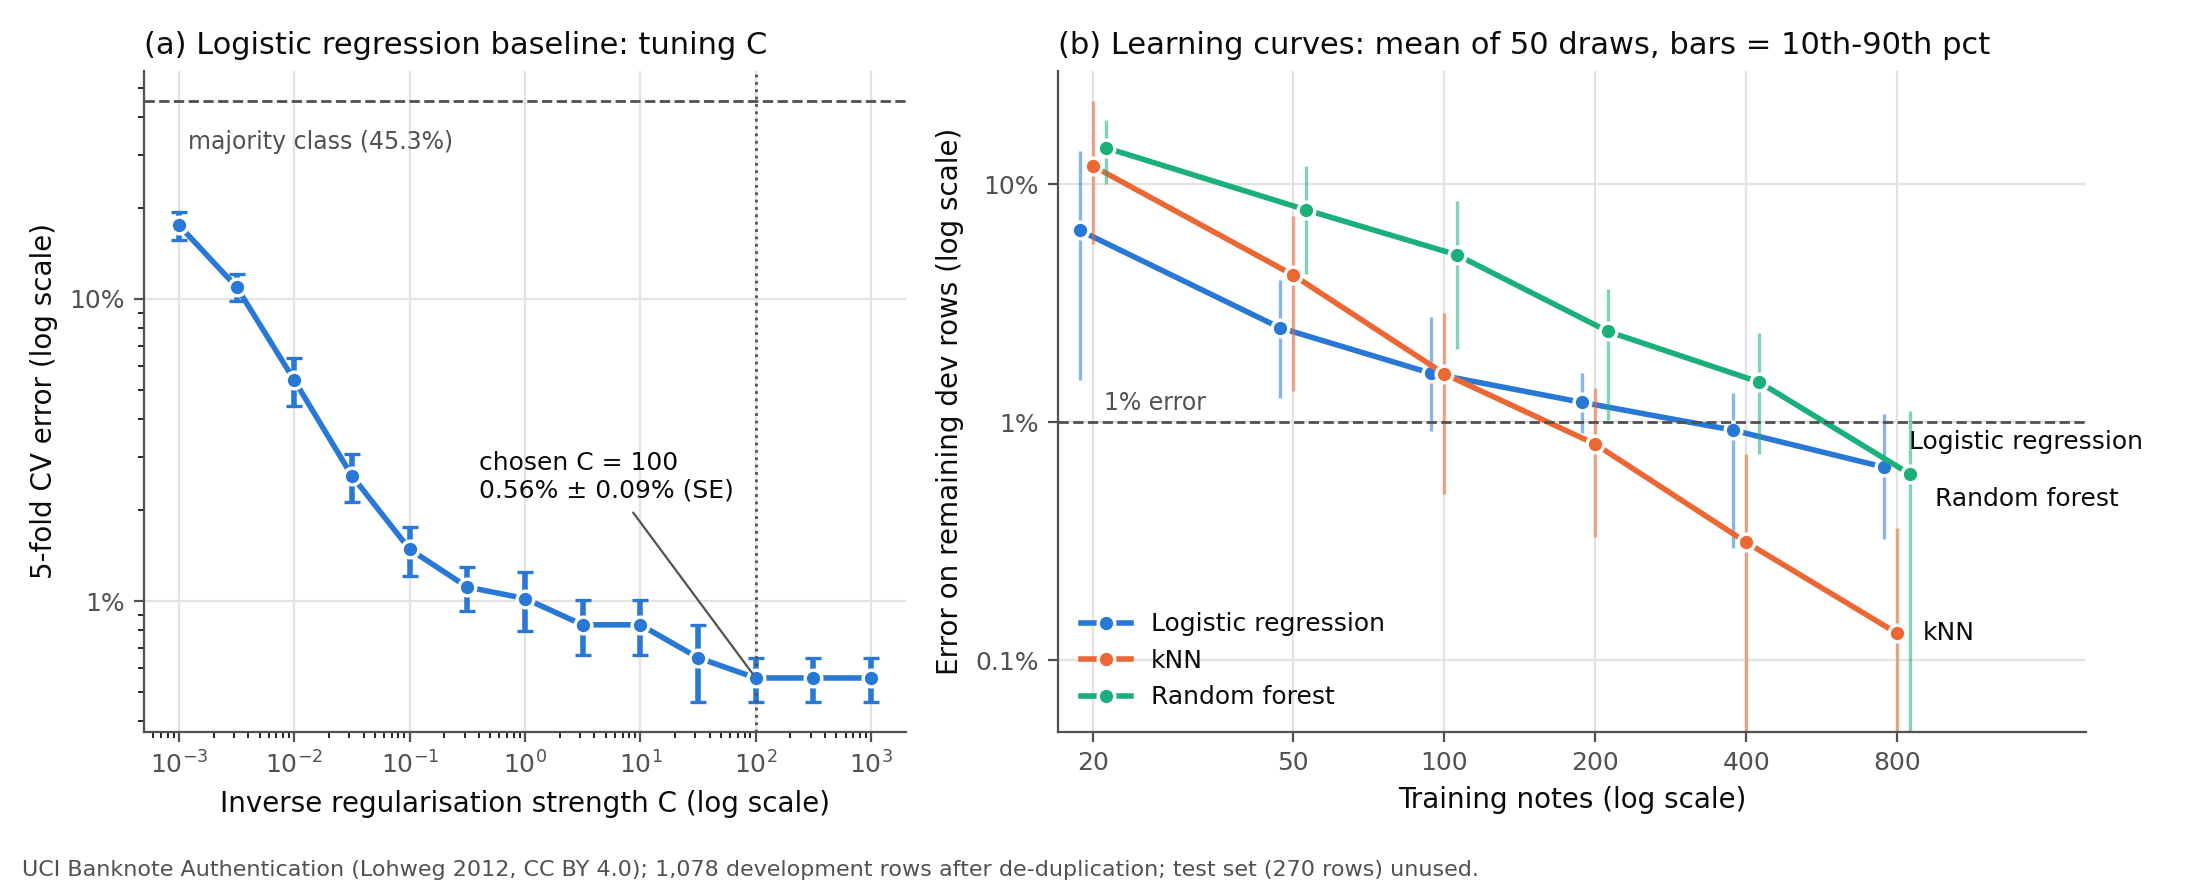
\includegraphics[width=\linewidth]{../figures/baseline.png}
  \caption{Baseline-checkpoint figure. (a) Logistic-regression CV error across the $C$ grid, $\pm$1 SE. (b) The first learning curves (three methods, six sizes); the main text extends these.}
  \label{fig:cgrid}
\end{figure}

\subsection{Full learning curves}
\label{app:full}
\begin{table}[H]
  \centering
  \caption{Mean error (\%) $\pm$ SE over 50 draws, scored on the development notes not used for training. Bold marks the lowest mean at each size. $^\dagger$Extension.}
  \label{tab:full}
  \small
  % generated by src/make_tables.py
\begin{tabular}{rccccc}
\toprule
$n$ & Logistic regression & $k$NN & Random forest$^\dagger$ & Gradient boosting$^\dagger$ & Neural network$^\dagger$ \\
\midrule
10 & 16.28 $\pm$ 1.51 & 21.57 $\pm$ 1.31 & 23.24 $\pm$ 1.47 & 21.00 $\pm$ 1.45 & \textbf{11.90 $\pm$ 1.41} \\
20 & 6.39 $\pm$ 0.85 & 11.89 $\pm$ 1.04 & 14.22 $\pm$ 0.71 & 15.68 $\pm$ 0.78 & \textbf{4.74 $\pm$ 0.51} \\
30 & 3.38 $\pm$ 0.33 & 7.11 $\pm$ 0.47 & 9.95 $\pm$ 0.52 & 11.70 $\pm$ 0.64 & \textbf{2.90 $\pm$ 0.34} \\
50 & 2.50 $\pm$ 0.20 & 4.15 $\pm$ 0.35 & 7.81 $\pm$ 0.45 & 8.92 $\pm$ 0.51 & \textbf{2.02 $\pm$ 0.20} \\
100 & 1.61 $\pm$ 0.11 & 1.60 $\pm$ 0.15 & 5.05 $\pm$ 0.34 & 5.34 $\pm$ 0.39 & \textbf{0.91 $\pm$ 0.10} \\
150 & 1.22 $\pm$ 0.07 & 0.99 $\pm$ 0.10 & 3.56 $\pm$ 0.23 & 3.13 $\pm$ 0.19 & \textbf{0.63 $\pm$ 0.08} \\
200 & 1.21 $\pm$ 0.06 & 0.81 $\pm$ 0.07 & 2.41 $\pm$ 0.15 & 1.91 $\pm$ 0.12 & \textbf{0.49 $\pm$ 0.06} \\
300 & 1.07 $\pm$ 0.06 & 0.56 $\pm$ 0.06 & 1.99 $\pm$ 0.12 & 1.88 $\pm$ 0.14 & \textbf{0.28 $\pm$ 0.05} \\
400 & 0.93 $\pm$ 0.05 & 0.31 $\pm$ 0.04 & 1.47 $\pm$ 0.09 & 1.17 $\pm$ 0.08 & \textbf{0.12 $\pm$ 0.03} \\
600 & 0.82 $\pm$ 0.06 & 0.13 $\pm$ 0.03 & 1.05 $\pm$ 0.07 & 0.66 $\pm$ 0.07 & \textbf{0.06 $\pm$ 0.02} \\
800 & 0.65 $\pm$ 0.06 & 0.13 $\pm$ 0.03 & 0.60 $\pm$ 0.06 & 0.33 $\pm$ 0.06 & \textbf{0.00 $\pm$ 0.00} \\
\bottomrule
\end{tabular}

\end{table}

\begin{table}[H]
  \centering
  \caption{Paired difference from logistic regression, in percentage points (negative is better than the baseline), with the number of draws (out of 50) in which the method beat / lost to the baseline; the rest are ties. Bold: $|\Delta|>2$ SE.}
  \label{tab:paired}
  \small
  \resizebox{\linewidth}{!}{% generated by src/make_tables.py
\begin{tabular}{lccccccc}
\toprule
$n$ & 10 & 20 & 50 & 100 & 200 & 400 & 800 \\
\midrule
$k$NN & \textbf{+5.28} (16/34) & \textbf{+5.50} (9/40) & \textbf{+1.66} (14/35) & $-$0.01 (27/19) & \textbf{$-$0.40} (37/9) & \textbf{$-$0.61} (45/0) & \textbf{$-$0.52} (41/2) \\
Random forest$^\dagger$ & \textbf{+6.96} (13/37) & \textbf{+7.83} (5/45) & \textbf{+5.31} (1/49) & \textbf{+3.44} (1/49) & \textbf{+1.19} (8/41) & \textbf{+0.55} (7/37) & $-$0.04 (21/20) \\
Gradient boosting$^\dagger$ & \textbf{+4.72} (18/32) & \textbf{+9.29} (6/44) & \textbf{+6.43} (1/49) & \textbf{+3.74} (0/50) & \textbf{+0.69} (12/34) & \textbf{+0.24} (15/30) & \textbf{$-$0.32} (34/9) \\
Neural network$^\dagger$ & \textbf{$-$4.39} (33/16) & \textbf{$-$1.65} (29/18) & \textbf{$-$0.47} (31/14) & \textbf{$-$0.70} (44/2) & \textbf{$-$0.72} (47/1) & \textbf{$-$0.81} (50/0) & \textbf{$-$0.65} (45/0) \\
\bottomrule
\end{tabular}
}
\end{table}

\begin{table}[H]
  \centering
  \caption{Most common hyperparameters chosen by inner CV, with the share of the 50 draws that chose them. For the forest, $m$ is the number of features tried per split.}
  \label{tab:params}
  \small
  \resizebox{\linewidth}{!}{% generated by src/make_tables.py
\begin{tabular}{lllll}
\toprule
Method & $n=10$ & $n=50$ & $n=200$ & $n=800$ \\
\midrule
Logistic regression & $C=0.001$ (38\%) & $C=3.16$ (30\%) & $C=1$ (26\%) & $C=100$ (42\%) \\
$k$NN & $k=1$ (80\%) & $k=1$ (68\%) & $k=1$ (80\%) & $k=1$ (98\%) \\
Random forest$^\dagger$ & $m=1$, leaf 1 (60\%) & $m=1$, leaf 1 (56\%) & $m=1$, leaf 1 (66\%) & $m=1$, leaf 1 (52\%) \\
Gradient boosting$^\dagger$ & $\eta=0.05$, depth 1 (84\%) & $\eta=0.05$, depth 1 (52\%) & $\eta=0.2$, depth 1 (50\%) & $\eta=0.2$, depth 3 (86\%) \\
Neural network$^\dagger$ & 8 units, $\alpha=0.0001$ (54\%) & 8 units, $\alpha=0.0001$ (50\%) & 8 units, $\alpha=0.0001$ (44\%) & 8 units, $\alpha=0.0001$ (72\%) \\
\bottomrule
\end{tabular}
}
\end{table}

\subsection{Grouped draws}
\label{app:grouped}
\begin{table}[H]
  \centering
  \caption{Mean error (\%) $\pm$ SE for random draws and for draws that keep each 8-row pseudo-specimen on one side of the split (training, inner CV folds and evaluation).}
  \label{tab:grouped}
  \small
  % generated by src/make_tables.py
\begin{tabular}{rcccc}
\toprule
 & \multicolumn{2}{c}{Logistic regression} & \multicolumn{2}{c}{$k$NN} \\
\cmidrule(lr){2-3}\cmidrule(lr){4-5}
$n$ & random & grouped & random & grouped \\
\midrule
50 & 2.50 $\pm$ 0.20 & 2.30 $\pm$ 0.28 & 4.15 $\pm$ 0.35 & 4.53 $\pm$ 0.44 \\
100 & 1.61 $\pm$ 0.11 & 1.86 $\pm$ 0.17 & 1.60 $\pm$ 0.15 & 1.57 $\pm$ 0.18 \\
200 & 1.21 $\pm$ 0.06 & 1.14 $\pm$ 0.04 & 0.81 $\pm$ 0.07 & 0.74 $\pm$ 0.06 \\
400 & 0.93 $\pm$ 0.05 & 0.96 $\pm$ 0.06 & 0.31 $\pm$ 0.04 & 0.30 $\pm$ 0.05 \\
800 & 0.65 $\pm$ 0.06 & 0.71 $\pm$ 0.08 & 0.13 $\pm$ 0.03 & 0.13 $\pm$ 0.03 \\
\bottomrule
\end{tabular}

\end{table}

\subsection{Random-forest tuning}
\label{app:forest}
\begin{table}[H]
  \centering
  \caption{Random forest on all development notes. Top: 5-fold CV error of the small grid used inside every draw against a 64-setting grid. Bottom: out-of-bag error against the number of trees ($m=2$).}
  \label{tab:forest}
  \small
  % generated by src/make_tables.py
\begin{tabular}{lrcl}
\toprule
Grid & Configs & CV error (\%) & Best setting \\
\midrule
small (used in curves) & 6 & 0.56 $\pm$ 0.27 & $m=2$, leaf 1, 200 trees \\
large & 64 & 0.46 $\pm$ 0.21 & $m=3$, leaf 1, 500 trees, gini \\
\bottomrule
\end{tabular}

\vspace{4pt}
\begin{tabular}{lrrrrrr}
\toprule
Trees & 25 & 50 & 100 & 200 & 500 & 1000 \\
\midrule
OOB error (\%) & 0.74 & 0.56 & 0.46 & 0.56 & 0.65 & 0.74 \\
\bottomrule
\end{tabular}

\end{table}

\subsection{Test-set ROC curves}
\label{app:roc}
\begin{figure}[H]
  \centering
  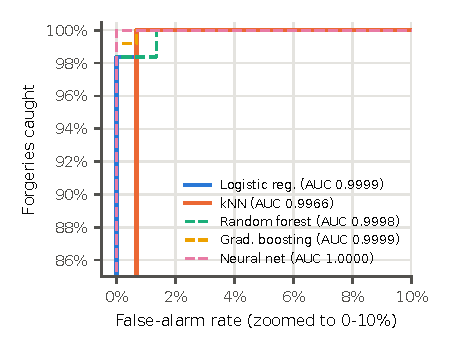
\includegraphics[width=0.55\linewidth]{../figures/test_roc.pdf}
  \caption{ROC curves on the 270 test notes, zoomed to the top-left corner.}
  \label{fig:roc}
\end{figure}

\section{Reproducibility}
\label{app:repro}
All code, the fixed split and the result files are at \url{https://github.com/maanasgoel/ese5420-banknote}. \texttt{src/baseline.py}, \texttt{src/learning\_curves.py}, \texttt{src/analyse.py} and \texttt{src/test\_eval.py} produce every number, and \texttt{src/make\_tables.py} writes every table and every number quoted in the text, so the paper cannot drift from the results. The full run takes about 20 minutes on an 8-core laptop (Python 3.10, scikit-learn 1.7.2).


\end{document}
